\documentclass{article}
\title{Notes for: Algorithms for Inverse Reinforcement Learning}
\author{-- \thanks{paper: https://ai.stanford.edu/~ang/papers/icml00-irl.pdf}}
\date{\today}
\usepackage{amsmath}
\usepackage{graphicx}
\usepackage{amsfonts}

\begin{document}
    \maketitle
    
    \section{High Level and Motivation}

    \subsection{Problem}
    
    \begin{itemize}
        \item Normal reinforcement learning is the process of extracting an optimal policy for a given reward function in an environment.
        \item Inverse reinforcement learning is the process of extracting a reward function from an environment given observed \textbf{optimal behavior}.
    \end{itemize}
    
    \subsection{Example}
    You are able to observe an agent's actions as it tackles a modified version of the Mountain Car problem:


    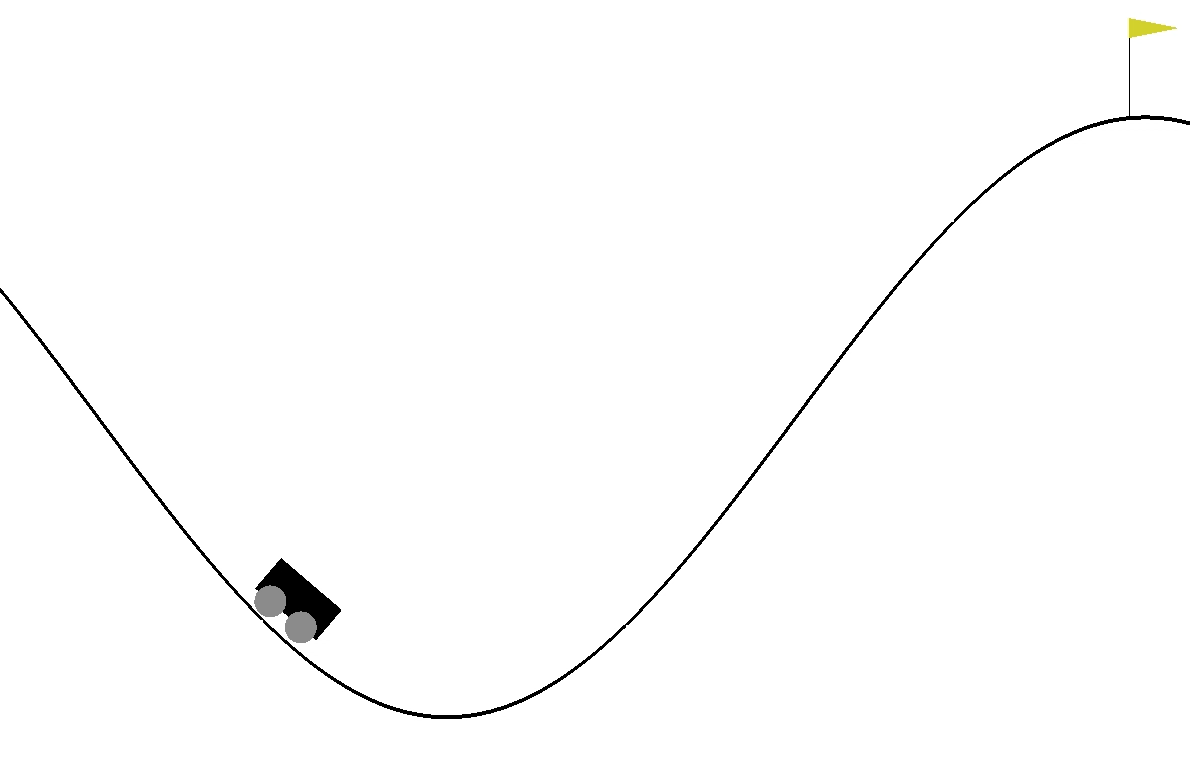
\includegraphics[width=7cm]{fig1.png}


    In the normal case, the car's aim is to reach the yellow flag where it will receive a reward.

    In the modified case, which interests us, the car driving agent was trained to reach a different location (unknown to us) by being provided a different reward signal. 

    We have access to:

    \begin{enumerate}
        \item the examples of the driving agent's actions over time
        \item the state before each decision was made, and
        \item a model of the environment
    \end{enumerate}

    Our goal is to uncover what the reward signal is.


    CRITICALLY: We assume that the actions we are observing are \textbf{optimal} for the reward function. In other words: We assume that the actions taken by the driver of the car are "perfect" so to speak, for the given reward function. 
    We then make inferences about possible reward functions, $R$, which satisfy the constraint that if an agent learns the optimal policy for $R$ it will exhibit the same behavior we observe in the driving examples provided. 


    \subsection{Identified issues}
    In any environment, with any observed action there exists multiple valid reward functions to explain the behavior. For example, in an environment which uniformly always gives 0 reward we can expect every policy in an environment with this $R$ to be "optimal". Such solutions to the IRL problem such as uniform reward functions are considered \emph{degenerate}.
    
    In order to select the "best" reward function $R$ is evaluated by how uniquely it describes the behavior exhibited. I.e. if $R$ can explain many different policies (think how the 0 reward solution explains every policy) then it is valued less.


    \subsection{Three Problem Areas}
    The paper highlights and provides solutions for 3 distinct types of environments and circumstances for IRL.
    \begin{enumerate} 
        \item Discrete environments where the policy is fully known (finite state space)
        \item Continuous environments where the policy is fully known (infinite state space)
        \item Continuous environments where you are only provided with a finite set of observed trajectories (infinite state space with limited information about the agent). This is the most realistic setting.
    \end{enumerate}

    \section{Core content}
    
    \subsection{Notation used by the paper}
    It's all pretty standard stuff:
    
    \begin{itemize}
        \item $S$ is a finite set of $N$ states
        \item $A = \{a_1, \dots, a_k\}$
        \item $P_{sa}(\cdot)$ are the state transition probabilities upon taking action $a$ in state $s$
        \item $\gamma \in [0,1)$ is the discount factor
        \item $R: S \mapsto \mathbb{R}$ is the reward function, bounded in absolute value by $R_{\max}$. They write the reward function as $R(s)$. 
        \item $\pi: S \mapsto A$ is a policy.
        \item $V^*(s) = \sup_\pi V^\pi (s)$ is the optimal value function
        \item $Q^*(s, a) = \sup_\pi Q^\pi (s, a)$ is the optimal Q-function
    \end{itemize}

    When looking at discrete problems, we represent the functions as \emph{vectors indexed by the state}.
    For example:
    $$\mathbf{I} = \mbox{identity}$$  
    $$\mathbf{R}[S_i] = \mbox{reward at $S_i$}$$  
    $$\mathbf{V}^\pi[S_i] = \mbox{value at $S_i$ while following policy $\pi$}$$  
    $$\mathbf{P}_a[S_i, S_j] = \mbox{starting in $S_i$, taking action $a$, probability of arriving in $S_j$ }$$  

    \subsection{Constraint on R}

    The following condition must hold if \textbf{R} is an optimal solution:
    $$(\mathbf{P}_{\pi(s)} - \mathbf{P}_a)(\mathbf{I} - \gamma \mathbf{P}_{\pi(s)})^{-1} \mathbf{R} \succeq 0 \;\;\;\;\; \forall \, a \in (A - \{\pi(s)\})$$
  
    $$x \succeq y \text{ if and only if } \forall i \; x_i \ge y_i$$

    $\pi(s)$ is the optimal action (what we observe) and therefore $a$ is every action other than the optimal action.

    This can be intuitively viewed with an example:


    $$
    \mathbf{P_{\pi(s)}} = \begin{bmatrix}
        0.2 & 0.8 \\
        0.5 & 0.5 
    \end{bmatrix}
    $$
    Where each row represents a possible starting state $[S_0 $ or $ S_1]$ and each column represents a possible next state $[S'_0 $ or $ S'_1]$ all given you take the action $\pi(s)$. The probability of transitioning from $S \to S'$ is the value in that cell.

    $$
    \mathbf{P}_{a_2} = \begin{bmatrix}
        0.9 & 0.1 \\
        0.7 & 0.3 
    \end{bmatrix}
    $$

    Where $a_2$ is an example of an action other than $\pi(s)$.

    $$
    \left (
    \begin{bmatrix}
        0.2 & 0.8 \\
        0.5 & 0.5 
    \end{bmatrix}
        -
    \begin{bmatrix}
        0.9 & 0.1 \\
        0.7 & 0.3 
    \end{bmatrix}
    \right ) 
    \left (
        \begin{bmatrix}
            1 & 0 \\
            0 & 1 
        \end{bmatrix}
        -
        \gamma
        \begin{bmatrix}
            0.2 & 0.8 \\
            0.5 & 0.5 
        \end{bmatrix}
    \right )^{-1}
    \begin{bmatrix}
        r_0 \\
        r_1 
    \end{bmatrix} \succeq 0 
    $$
    \begin{center}
        let $\gamma = 0.8$ 
    \end{center} 
    $$
    \begin{bmatrix}
        -0.6 & 0.7 \\
        -0.2 & 0.2 
    \end{bmatrix} 
        \begin{bmatrix}
            0.79 & 0.84 \\
            0.53 & 1.11 
        \end{bmatrix}
    \begin{bmatrix}
        r_0 \\
        r_1 
    \end{bmatrix} \succeq 0 
    $$
    
    If we let $r_0 = 1$ and $r_1 = 0$ (arbitrarily chosen) meaning that in state $S_0$ the agent receives 1 reward and in state $S_1$ the agent receives 0 reward. Any policy which maximises getting to state $S_0$ will be preferable (better).
    
    $$
    \begin{bmatrix}
        -0.6 & 0.7 \\
        -0.2 & 0.2 
    \end{bmatrix} 
        \begin{bmatrix}
            0.79 & 0.84 \\
            0.53 & 1.11 
        \end{bmatrix}
    \begin{bmatrix}
        1 \\
        0 
    \end{bmatrix} \succeq 0 
    $$
    $$
    \begin{bmatrix}
        -0.103 \\
        -0.052 
    \end{bmatrix} \not \succeq 
    \begin{bmatrix}
        0 \\
        0 
    \end{bmatrix}
    $$

    Looking at our result we can see that the parameters $r_0=1$ and $r_1=0$ do not satisfy the condition. This makes logical sense as: 
    
    $$
    \mathbf{P_{\pi(s)}} = \begin{bmatrix}
        0.2 & 0.8 \\
        0.5 & 0.5 
    \end{bmatrix}
    $$
    $$
    \mathbf{P}_{a_2} = \begin{bmatrix}
        0.9 & 0.1 \\
        0.7 & 0.3 
    \end{bmatrix}
    $$
    and we can see that 
    
    $\pi(s)$ will (with probability $\frac{0.2+0.5}{2} = 0.35$) will leave the agent in $S_0$  and
    
    $a_2$ will (with probability $\frac{0.9+0.7}{2} = 0.8$) leave the agent in $S_0$.

    So: $\pi(s)$ will perform worse than $a_2$ when $r_0 > r_1$. Therefore in this case, our selection of $\mathbf{R}$ was poor.
    It's important to note, $\pi(s)$ should be the optimal action meaning, there are no other better actions which is where the $\forall \, a \in (A - \{\pi(s)\})$ component of the original equation comes from.

    At this point it's also clear why the degenerate solution $\mathbf{R} = 0$ exists.

    \subsection{The unique optimal policy}
    By replacing all of the inequalities above with strict inequalities:
    $$(\mathbf{P}_{\pi(s)} - \mathbf{P}_a)(\mathbf{I} - \gamma \mathbf{P}_{\pi(s)})^{-1} \mathbf{R} \succ 0$$
    We can see that this strict inequaliy will yield $\pi(s)$ as the \emph{unique} optimal policy for $\mathbf{R}$ meaning that degenerate solutions such as $\mathbf{R} = 0$ are removed. This, however, does not exclude the fact that there can be multiple valid $\mathbf{R}$s per $\pi(s)$.

    \textbf{Before:}
    \begin{itemize}
        \item Many valid $\pi(s)$ per $\mathbf{R}$ and
        \item Many valid $\mathbf{R}$s per $\pi(s)$
    \end{itemize}

    \textbf{After:} 
    \begin{itemize}
        \item 1 valid $\pi(s)$ per $\mathbf{R}$ an
        \item Many valid $\mathbf{R}$s per $\pi(s)$
    \end{itemize}

    The next question may be:

    \dots
    How do we pick the most valid $\mathbf{R}$?

    \subsection{Picking R}
   
    \subsubsection{How to evaluate different valid $\mathbf{R}$s}

    The paper considers two things when evaluating:
    \begin{enumerate}
        \item Demand that it makes $\pi$ optimal (this one's pretty obvious because if it didn't we wouldn't be solving the IRL problem)
        \item Select an $\mathbf{R}$ which optimizes $\pi$ but minimizes other policies.
    \end{enumerate}
    
    The paper presents an option for achieving (2.). We can evaluate $\mathbf{R}$s using the following:

    $$\sum_{s \in S} \left ( Q^\pi (s, \pi(s)) - \max_{a \in \left(A - \pi(s)\right)} Q^\pi (s, a) \right)$$

    
    In plain english:

    
    We find the value of following the policy $\pi$ given $\mathbf{R}$. We then subtract the the value of picking the best action out of the remaining actions - \emph{we exclude the one $\pi$ picks}.
    IF $\pi$ is optimal then the value being subtracted will always be the value of the second best action (\emph{because $\pi$ picks the best one}).
    
    Simply performing this over every action will present you with a measure for evaluating different $\mathbf{R}$s.
        
        
    \subsubsection{"Overfitting" $\mathbf{R}$}

    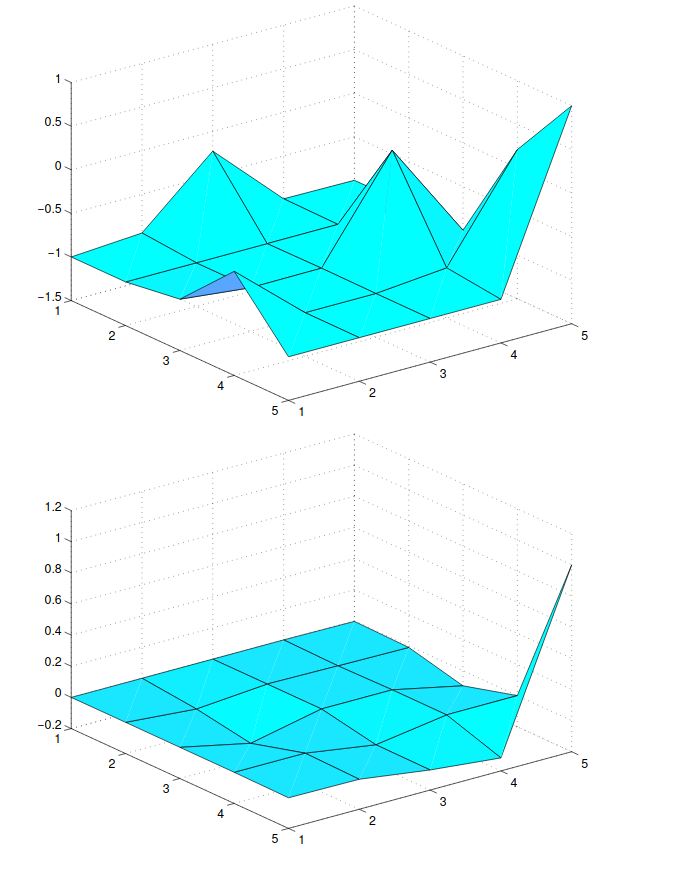
\includegraphics[width=7cm]{fig2.png}
        \textbf{Top: recovered R with small $\lambda$ Bottom: recovered R with large $\lambda$}
    


    Although our goal is to extract an exact reward function there may still be issues with whether we will extract the true reward function.
    
    For example, in a state where the policy must make an arbitrary decision (say: move up or move down) and the same decision is made each time. We may learn an incorrect reward function even though the agent was acting optimally.

    They suggest a general solution to this and other related problems by introducing a penalty function $-\lambda ||\mathbf{R}||$. The paper proposes that solutions with smaller rewards are "simpler".

    


    \subsubsection{How to actually pick your $\mathbf{R}$}

    Just solve the following linear programming task:

    \textbf{(what is LP?):}

    Linear programming (LP, also called linear optimization) is a method to achieve the best outcome (such as maximum profit or lowest cost) in a mathematical model whose requirements are represented by linear relationships. Linear programming is a special case of mathematical programming (also known as mathematical optimization). 

    $$\text{maximise} \sum_{i=1}^N \min_{a \in \{ a_2, \dots, a_k \}} (P_{\pi(s)}(i)- P_a(i)) (I - \gamma P_{\pi(s)})^{-1} R - \gamma ||R||_1$$
    $$s.t. (P_{\pi(s)} - P_a)(I - \gamma P_{a_1})^{-1} R \succeq 0 \;\;\;\; \forall a \in (A - \pi(s)) $$
    $$|R_i| \le R_{\max}, i = 1, \dots, N$$

    We can see each element that has been discussed so far:
    $$(P_{\pi(s)} - P_a)(I - \gamma P_{a_1})^{-1} R \succeq 0 \;\;\;\; \forall a \in (A - \pi(s)) $$
    Is the constraint for $\mathbf{R}$ to be optimal. 

    $$\text{maximise} \sum_{i=1}^N \min_{a \in \{ a_2, \dots, a_k \}} (P_{\pi(s)}(i)- P_a(i)) (I - \gamma P_{\pi(s)})^{-1} R - \gamma ||R||_1$$
    Is the optimization of $\mathbf{R}$ using 2.4.1 and 2.4.2
    
    $$|R_i| \le R_{\max}, i = 1, \dots, N$$
    Is one of the initial constraints of the problem (that the rewards are bounded by some $R_{\max}$)



    \section{Their Experiments and Comments}

    They don't actually provide any data for their experiments and this paper was published in 2000. There are more modern approaches to extracting reward signals. For example, using a GAN to estimate a user's behavior can be then used to make inference about their preferences based on their actions https://arxiv.org/abs/1812.10613.

    \subsection{5x5 Grid world}    

    \begin{itemize}
        \item Start in the lower left cell of a 5x5 grid
        \item The top right cell is an absorbing state where the agent receives 1 reward
        \item The environment is stochastic, there is a 30\% chance that the action chosen will be randomized resulting in a random movement instead.
        
        

    \end{itemize}

    \subsection{Mountain car}

    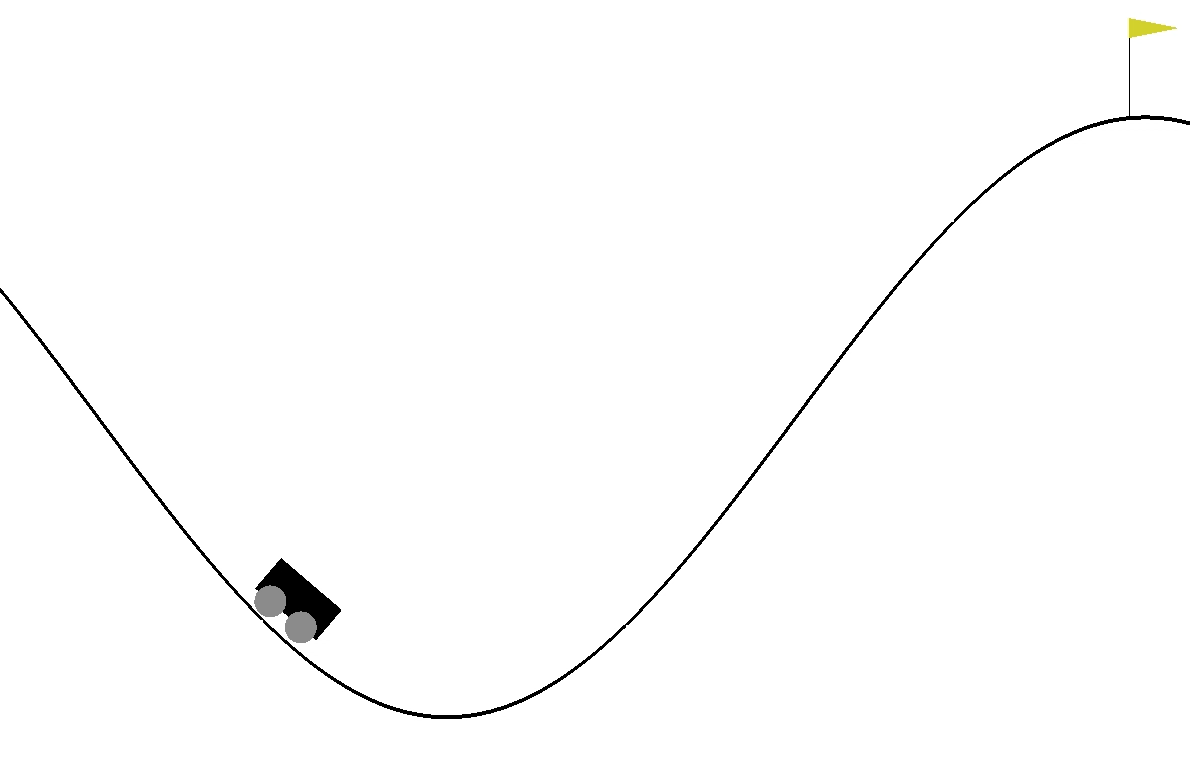
\includegraphics[width=7cm]{fig1.png}
    
    \begin{itemize}
        \item -1 reward per step until the car reaches the terminal point.
        \item Movements are continuous
    \end{itemize}

    \subsection{Sample based, continuous 5x5 Grid world}

    \begin{itemize}
        \item Modified version of the 5x5 grid world where the environment is continuous: The state was  $[0,1] \times [0,1]$.
        \item The environment is still stochastic as after each action, noise $[-0.1, 0.1]$ is added.
        \item We only have access to trajectories of actions rather than direct access to the policy.
    \end{itemize}

\end{document}